\documentclass[a4paper,14pt,href]{article}

% Используем нестандартный размер шрифта
\usepackage{extsizes}

% Делаем отступ для первого параграфа
\usepackage{indentfirst}

% Для поддержки поиска по pdf документу
\usepackage{cmap}

% Поддержка кириллицы
\usepackage[T2A]{fontenc}
\usepackage[utf8]{inputenc}
\usepackage[english,russian]{babel}

% Поддержка списков
\usepackage{enumerate}

% Заменяем библиографию с квадратных скобок на точку
\makeatletter
\renewcommand{\@biblabel}[1]{#1.}
\makeatother

% Графический пакет
\usepackage{graphicx}
\usepackage{epstopdf}
\usepackage{tikz}

% Математические шрифты AMS
\usepackage{amstext, amssymb, amsmath}

% В заголовках появляется точка, но при ссылке на них ее нет
\usepackage{misccorr}

% Поддержка гиперссылок
\usepackage{url}

% Задаем полуторный межстрочный интервал
\linespread{1.3}

% Задаем глубину оглавления
\setcounter{tocdepth}{2}

% Путь к изображениям, по умолчанию
\graphicspath{{images/}}

% Задаем отступ абзаца
\setlength{\parindent}{1.25cm}

\renewcommand{\labelenumi}{\arabic{enumi}.}% Меняем везде перечисления на цифра.цифра

% Меняем поля страницы
\usepackage{geometry}
\geometry{left=2.5cm}   % левое поле
\geometry{right=2.5cm}  % правое поле
\geometry{top=2.5cm}    % верхнее поле
\geometry{bottom=2.5cm} % нижнее поле

\begin{document}


%%%
% Титульный лист
%%%
\thispagestyle{empty}
\begin{center}
Федеральное государственное автономное образовательное учреждение \\
высшего профессионального образования \\
\textsc{<<Южный Федеральный Университет>>}\\[1.0cm]

Факультет математики, механики и компьютерных наук\\[1.0cm]

Направление подготовки 010400 \\
<<Прикладная математика и информатика>>\\[3cm]

А. А. Тактаров \\[1.0cm]
\textsc{Реактивный фреймворк для организациии мультиагентных распределенных вычислений}\\[1.0cm]

\textit{Магистерская диссертация}\\[2.0cm]

\begin{flushright}
    Научный руководитель: \\
    старший преподаватель \\
    В. Н. Брагилевский \\[1.0cm]

    Рецензент: \\
    доцент, к. ф.-м. н.\\
    С. А. Гуда
\end{flushright}

\vfill

  Ростов-на-Дону\\
  2014
\end{center}

\newpage
\tableofcontents

\newpage
\section*{Введение}
\addcontentsline{toc}{section}{Введение}

Стремительный рост возможностей технологий беспроводной передачи данных, а также широкое распространение мобильных и встраиваемых устройств
способоствовали появлению концепции так называемого <<Интернета вещей>> (англ. \textit{<<Internet of Things>>})\cite{IoTWired}, которая заключается в объединении всех окружающих нас вещей в огромную вычислительную сеть. Участниками (\textit{агентами}) такой сети являются устройства, которые способны собирать информацию о физической среде, обрабатывать ее и реагировать на изменение состояния других агентов и всей системы в целом. Стабильное функционирование такой сети позволит с огромной скоростью внедрять и использовать такие технологии, как <<умные>> датчики\cite{NestThermostat}, носимые устройства (англ. \textit{wearable devices}), а также системы автоматизированного управления домом. Кроме того, становление <<Интернета вещей>> влечет за собой появление принципиально новых потоков информации, тщательный анализ которых позволит улучшать существующие системы здравоохранения, безопасности и контролировать состояние окружающей среды.

Однако, создание подобного рода сети невозможно без наличия функционирующей инфраструктуры, которая бы позволила быстро и эффективно интегрировать новые компоненты. Исходя из распределенной природы описываемой сети, сформулируем необходимые для этого требования:

\begin{enumerate}
  \item Соблюдение принципа системности при разработке\cite{SystemPrinciple}. Продукт должен быть представлен в виде целой системы компонентов, каждый из которых обладает определенной функцией. Такие компоненты автоматически становятся автономными участниками сети.

  \item Однородность среды. Компоненты сети должны иметь возможность взаимодействовать между собой, используя стандартизированные протоколы и схемы. Задачи идентификации, обеспечения целостности, конфиденциальности передаваемых данных должны по возможности быть решены этими протоколами.

  \item Открытость используемых технологий. Применение как программных, так и аппаратных решений, которые имеют открытую документацию, лояльные  условия использования и одновременно поддерживаются разными разработчиками (обычно целым сообществом), позволяет в определенных случаях решить проблему интеграции компонентов и сократить разрыв между разработкой и запуском в производство. Кроме того, открытые платформы предоставляют широкие возможности для начинающих команд разработчиков, что является благоприятным для формирования рынка.
\end{enumerate}

В данной работе описан процесс реализации и интеграции муль\-тиагентной системы на примере задачи распределенной печати фотографий. В рамках разработанной системы устройство, печатающее фотографию, рассматривается как автономный агент, который обладает состоянием и способен принимать и исполнять задания. Принципы, сформулированные выше, были использованы в качестве основополагающих на этапах проектирования и разработки данного продукта.

\newpage
\section{Постановка задачи}
Целью работы является разработка и развертывание системы, позволяющей организовать моментальную печать фотографий пользователей социальной сети Instagram, распределяя задания печати среди подключенных к системе агентов -- \textit{печатных станций}, в состав которых входит печатное устройство -- принтер.

<<Здесь краткое описание цикла работы>>

Сформулируем основные требования, предъявляемые к системе:
\begin{enumerate}
  \item Печатные станции могут быть физически отделены друг от друга, кроме того они могут находиться в разных сегментах сети. Необходим способ
    организации канала связи между агентами и контроль жизнеспособности этого канала.

  \item Необходим интерфейс управления печатными станциями и заданиями печати.

  \item Система должна иметь минимальный отклик и максимально быстро реагировать на изменение состояния компонентов. Изменение статуса задания печати (печать может завершиться успешно, а может закончиться неудачей в результате обрыва соединения) должно моментально отражаться в интерфейсе управления заданиями.


\end{enumerate}

\begin{figure}[htbp]
\begin{center}
  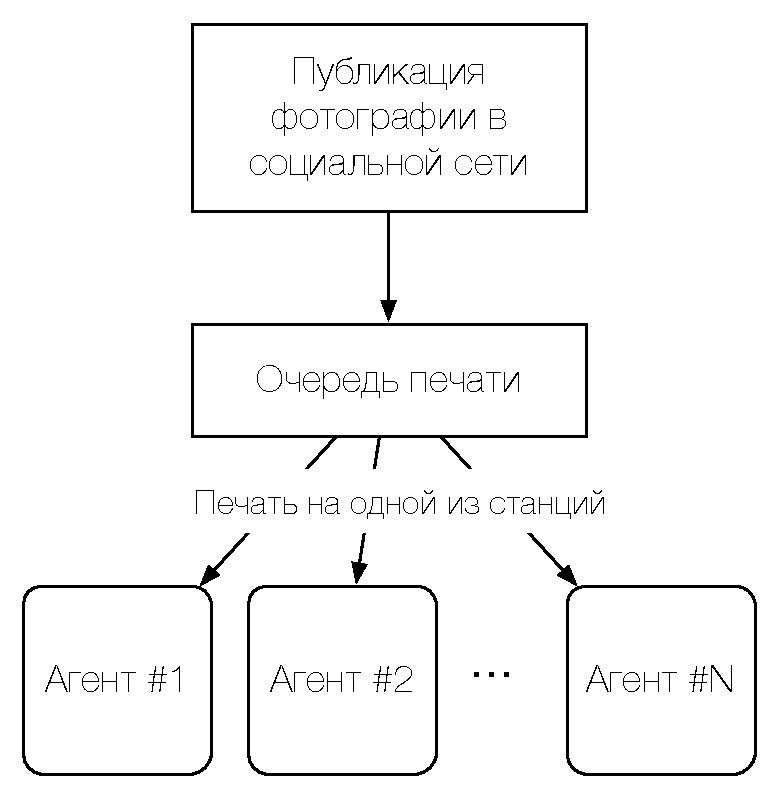
\includegraphics[scale=0.7]{print_schema.pdf}
    \caption{Архитектура разработанного приложения}
    \label{fig:Architecture}
\end{center}
\end{figure}



\newpage
\addcontentsline{toc}{section}{Список литературы}

\bibliographystyle{unsrt}
\bibliography{bibliography/sources}

\end{document}
